\documentclass{standalone}
\usepackage{tikz}
\usetikzlibrary{patterns, positioning}


\begin{document}
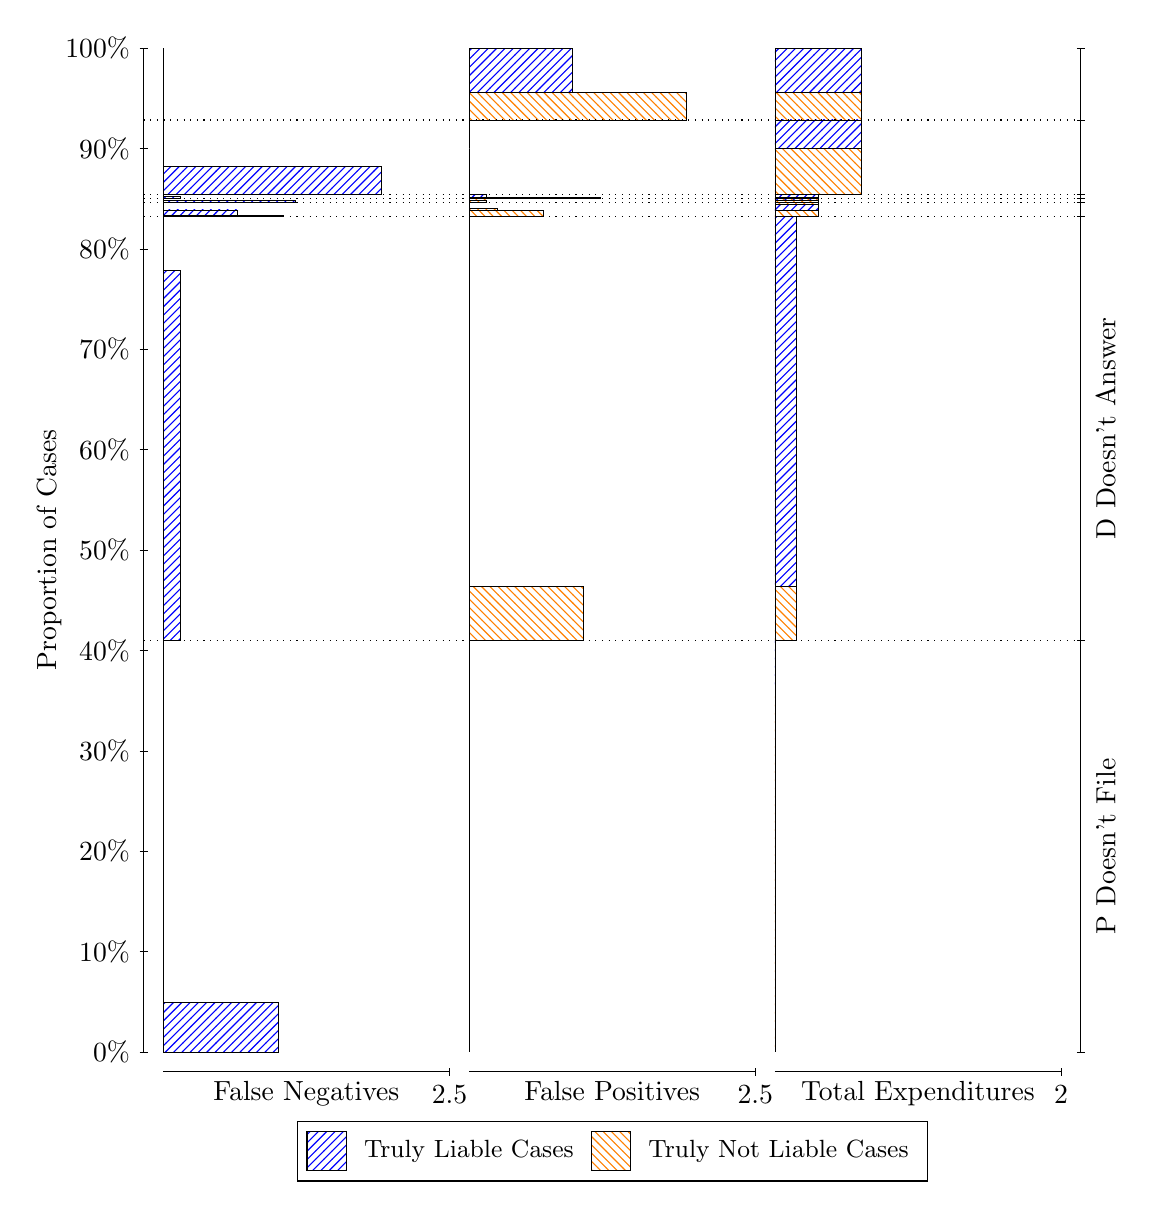
\begin{tikzpicture}
\draw[black, very thin] (1.5,1.75) -- (1.5,14.5);
\node[rotate=90, text=black, anchor=center] at (0.3, 8.125) {Proportion of Cases};
\draw[black, very thin] (1.45,1.75) -- (1.55,1.75);
\node[text=black, anchor=east] at (1.45, 1.75) {0\%};
\draw[black, very thin] (1.45,3.025) -- (1.55,3.025);
\node[text=black, anchor=east] at (1.45, 3.025) {10\%};
\draw[black, very thin] (1.45,4.3) -- (1.55,4.3);
\node[text=black, anchor=east] at (1.45, 4.3) {20\%};
\draw[black, very thin] (1.45,5.575) -- (1.55,5.575);
\node[text=black, anchor=east] at (1.45, 5.575) {30\%};
\draw[black, very thin] (1.45,6.85) -- (1.55,6.85);
\node[text=black, anchor=east] at (1.45, 6.85) {40\%};
\draw[black, very thin] (1.45,8.125) -- (1.55,8.125);
\node[text=black, anchor=east] at (1.45, 8.125) {50\%};
\draw[black, very thin] (1.45,9.4) -- (1.55,9.4);
\node[text=black, anchor=east] at (1.45, 9.4) {60\%};
\draw[black, very thin] (1.45,10.675) -- (1.55,10.675);
\node[text=black, anchor=east] at (1.45, 10.675) {70\%};
\draw[black, very thin] (1.45,11.95) -- (1.55,11.95);
\node[text=black, anchor=east] at (1.45, 11.95) {80\%};
\draw[black, very thin] (1.45,13.225) -- (1.55,13.225);
\node[text=black, anchor=east] at (1.45, 13.225) {90\%};
\draw[black, very thin] (1.45,14.5) -- (1.55,14.5);
\node[text=black, anchor=east] at (1.45, 14.5) {100\%};

\draw[black, very thin] (13.4,1.75) -- (13.4,14.5);
\draw[black, very thin] (13.35,1.75) -- (13.45,1.75);
\node[anchor=west] at (13.35, 1.75) {};
\draw[black, very thin] (13.35,6.9758) -- (13.45,6.9758);
\node[anchor=west] at (13.35, 6.9758) {};
\draw[black, very thin] (13.35,12.366) -- (13.45,12.366);
\node[anchor=west] at (13.35, 12.366) {};
\draw[black, very thin] (13.35,12.543) -- (13.45,12.543);
\node[anchor=west] at (13.35, 12.543) {};
\draw[black, very thin] (13.35,12.59) -- (13.45,12.59);
\node[anchor=west] at (13.35, 12.59) {};
\draw[black, very thin] (13.35,12.637) -- (13.45,12.637);
\node[anchor=west] at (13.35, 12.637) {};
\draw[black, very thin] (13.35,13.586) -- (13.45,13.586);
\node[anchor=west] at (13.35, 13.586) {};
\draw[black, very thin] (13.35,14.5) -- (13.45,14.5);
\node[anchor=west] at (13.35, 14.5) {};

\draw[black, very thin, pattern color=blue, pattern=north east lines] (1.75,1.75) rectangle (3.2033,2.3764);
\draw[black, very thin, pattern color=orange, pattern=north west lines] (1.75,2.3764) rectangle (1.75,6.9758);
\draw[black, very thin, pattern color=blue, pattern=north east lines] (1.75,6.9758) rectangle (1.968,11.68);
\draw[black, very thin, pattern color=orange, pattern=north west lines] (1.75,11.68) rectangle (1.75,12.366);
\draw[black, very thin, pattern color=blue, pattern=north east lines] (1.75,12.366) rectangle (3.276,12.372);
\draw[black, very thin, pattern color=blue, pattern=north east lines] (1.75,12.372) rectangle (2.6947,12.444);
\draw[black, very thin, pattern color=orange, pattern=north west lines] (1.75,12.444) rectangle (1.75,12.543);
\draw[black, very thin, pattern color=blue, pattern=north east lines] (1.75,12.543) rectangle (3.4213,12.561);
\draw[black, very thin, pattern color=orange, pattern=north west lines] (1.75,12.561) rectangle (1.75,12.59);
\draw[black, very thin, pattern color=blue, pattern=north east lines] (1.75,12.59) rectangle (1.968,12.618);
\draw[black, very thin, pattern color=orange, pattern=north west lines] (1.75,12.618) rectangle (1.75,12.637);
\draw[black, very thin, pattern color=blue, pattern=north east lines] (1.75,12.637) rectangle (4.5113,12.998);
\draw[black, very thin, pattern color=orange, pattern=north west lines] (1.75,12.998) rectangle (1.75,13.586);
\draw[black, very thin, pattern color=orange, pattern=north west lines] (1.75,13.586) rectangle (1.75,13.941);
\draw[black, very thin, pattern color=blue, pattern=north east lines] (1.75,13.941) rectangle (1.75,14.5);
\draw[black, very thin, pattern color=orange, pattern=north west lines] (5.6333,1.75) rectangle (5.6333,6.3495);
\draw[black, very thin, pattern color=blue, pattern=north east lines] (5.6333,6.3495) rectangle (5.6333,6.9758);
\draw[black, very thin, pattern color=orange, pattern=north west lines] (5.6333,6.9758) rectangle (7.0867,7.6617);
\draw[black, very thin, pattern color=blue, pattern=north east lines] (5.6333,7.6617) rectangle (5.6333,12.366);
\draw[black, very thin, pattern color=orange, pattern=north west lines] (5.6333,12.366) rectangle (6.578,12.438);
\draw[black, very thin, pattern color=orange, pattern=north west lines] (5.6333,12.438) rectangle (5.9967,12.465);
\draw[black, very thin, pattern color=blue, pattern=north east lines] (5.6333,12.465) rectangle (5.6333,12.543);
\draw[black, very thin, pattern color=orange, pattern=north west lines] (5.6333,12.543) rectangle (5.8513,12.572);
\draw[black, very thin, pattern color=blue, pattern=north east lines] (5.6333,12.572) rectangle (5.6333,12.59);
\draw[black, very thin, pattern color=orange, pattern=north west lines] (5.6333,12.59) rectangle (7.3047,12.608);
\draw[black, very thin, pattern color=blue, pattern=north east lines] (5.6333,12.608) rectangle (5.8513,12.637);
\draw[black, very thin, pattern color=orange, pattern=north west lines] (5.6333,12.637) rectangle (5.6333,13.225);
\draw[black, very thin, pattern color=blue, pattern=north east lines] (5.6333,13.225) rectangle (5.6333,13.586);
\draw[black, very thin, pattern color=orange, pattern=north west lines] (5.6333,13.586) rectangle (8.3947,13.941);
\draw[black, very thin, pattern color=blue, pattern=north east lines] (5.6333,13.941) rectangle (6.9413,14.5);
\draw[black, very thin, pattern color=orange, pattern=north west lines] (9.5167,1.75) rectangle (9.5167,6.3495);
\draw[black, very thin, pattern color=blue, pattern=north east lines] (9.5167,6.3495) rectangle (9.5167,6.9758);
\draw[black, very thin, pattern color=orange, pattern=north west lines] (9.5167,6.9758) rectangle (9.7892,7.6617);
\draw[black, very thin, pattern color=blue, pattern=north east lines] (9.5167,7.6617) rectangle (9.7892,12.366);
\draw[black, very thin, pattern color=orange, pattern=north west lines] (9.5167,12.366) rectangle (10.062,12.438);
\draw[black, very thin, pattern color=blue, pattern=north east lines] (9.5167,12.438) rectangle (10.062,12.511);
\draw[black, very thin, pattern color=orange, pattern=north west lines] (9.5167,12.511) rectangle (10.062,12.537);
\draw[black, very thin, pattern color=blue, pattern=north east lines] (9.5167,12.537) rectangle (10.062,12.543);
\draw[black, very thin, pattern color=orange, pattern=north west lines] (9.5167,12.543) rectangle (10.062,12.572);
\draw[black, very thin, pattern color=blue, pattern=north east lines] (9.5167,12.572) rectangle (10.062,12.59);
\draw[black, very thin, pattern color=orange, pattern=north west lines] (9.5167,12.59) rectangle (10.062,12.608);
\draw[black, very thin, pattern color=blue, pattern=north east lines] (9.5167,12.608) rectangle (10.062,12.637);
\draw[black, very thin, pattern color=orange, pattern=north west lines] (9.5167,12.637) rectangle (10.607,13.225);
\draw[black, very thin, pattern color=blue, pattern=north east lines] (9.5167,13.225) rectangle (10.607,13.586);
\draw[black, very thin, pattern color=orange, pattern=north west lines] (9.5167,13.586) rectangle (10.607,13.941);
\draw[black, very thin, pattern color=blue, pattern=north east lines] (9.5167,13.941) rectangle (10.607,14.5);
\draw[black, dotted] (1.5,6.9758) -- (13.4,6.9758);
\draw[black, dotted] (1.5,12.366) -- (13.4,12.366);
\draw[black, dotted] (1.5,12.543) -- (13.4,12.543);
\draw[black, dotted] (1.5,12.59) -- (13.4,12.59);
\draw[black, dotted] (1.5,12.637) -- (13.4,12.637);
\draw[black, dotted] (1.5,13.586) -- (13.4,13.586);
\draw[black, very thin] (1.75,1.5) -- (5.3833,1.5);
\node[text=black, anchor=north] at (3.5667, 1.5) {False Negatives};
\draw[black, very thin] (5.3833,1.45) -- (5.3833,1.55);
\node[text=black, anchor=north] at (5.3833, 1.45) {2.5};

\draw[black, very thin] (5.6333,1.5) -- (9.2667,1.5);
\node[text=black, anchor=north] at (7.45, 1.5) {False Positives};
\draw[black, very thin] (9.2667,1.45) -- (9.2667,1.55);
\node[text=black, anchor=north] at (9.2667, 1.45) {2.5};

\draw[black, very thin] (9.5167,1.5) -- (13.15,1.5);
\node[text=black, anchor=north] at (11.333, 1.5) {Total Expenditures};
\draw[black, very thin] (13.15,1.45) -- (13.15,1.55);
\node[text=black, anchor=north] at (13.15, 1.45) {2};

\node[text=black, centered, rotate=90] at (13.72, 4.3629) {P Doesn't File};
\node[text=black, centered, rotate=90] at (13.72, 9.6709) {D Doesn't Answer};






\draw (7.449999999999999,1.5) node[draw=none] (baseCoordinate) {};
\begin{scope}[align=center]
        \matrix[scale=0.5, draw=black, below=0.5cm of baseCoordinate, nodes={draw}, column sep=0.1cm]{
            \node[rectangle, draw, minimum width=0.5cm, minimum height=0.5cm, pattern color=blue, pattern=north east lines] {}; &
            \node[draw=none, font=\small, text=black] (B) {Truly Liable Cases}; &
            \node[rectangle, draw, minimum width=0.5cm, minimum height=0.5cm, pattern color=orange, pattern=north west lines] {}; &
            \node[draw=none, font=\small, text=black] (B) {Truly Not Liable Cases}; \\
            };
\end{scope}

\end{tikzpicture}
\end{document}